\documentclass[a4paper,12pt]{article}
\usepackage{amsmath}
\usepackage{amssymb}
\usepackage{amsfonts}
\usepackage{txfonts}
\usepackage{graphicx}
\usepackage[compress]{cite}
\newcommand{\mvec}[1]{\textbf{\textit{#1}}}

\title{Manual\\ \large for SpectrumMeasurement program\\ ver. 0.1}
\author{Yunsong Zhao}
\date{}
\begin{document}
\maketitle
\section{Introduction}
The SpectrumMeasurement program is used to measure the LI and IV curve of laser diodes
using current source, temperature controller and power meter. All the
instruments are wrapped in according matlab classes. 
\section{Usage}
The program can be called through the command ``SpectrumMeasurement'' in Matlab. Make
sure the classes of all the instruments that you are going to use are in the
same directory as ``SpectrumMeasurement.m'' or can be accessed by Matlab through
pathdef. If everything goes well, the first window you can get is shown in
Fig.~\ref{fig:setup}
\begin{figure}[htbp]
	\centering
	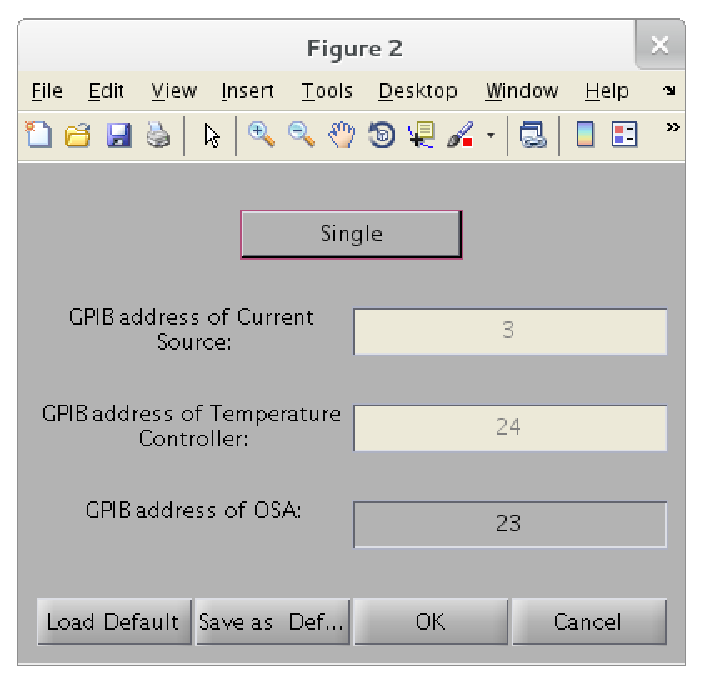
\includegraphics[width=0.5\textwidth]{./figs/setup.eps}
	\caption{SpectrumMeasurement Setup}
	\label{fig:setup}
\end{figure}

You can use the OSA along with current source and temperature controller or use
the OSA alone. This is controlled by the toggle button ``Single''. Now the
toggle button is not pressed and is shown ``Single''. In this mode, the ``GPIB
address of Current Source'' and ``GPIB address of Temperature Controller'' are
disabled. If you want to use current source and temperature controller as well,
just press down ``Single'' toggle button. Then the ``GPIB address of Current
Source'' and ``GPIB address of Temperature Controller'' text edits will be
enabled and ``Single'' text will change to ``Full''. The ``Load Default'' button
is used to load the default parameters to overwrite the current parameters. The
default setup is restored every time when the program is called. The ``Save as
Default'' button is used to save the current parameters as the default setup.
The ``OK'' button is used to accept the current parameters and continue to next
window. The ``Cancel'' button is used to exit the program.

After the ``OK'' button is pressed to accept the parameters, the
Fig.~\ref{fig:main_window} will be shown.

There are three panels in this window. Each panel represents an equipment and is
plotted and controlled by the according class. The equipment name is shown in
the title region of each panel. In Fig.~\ref{fig:main_window}, you can find
``ILX3744B Continuous Current Source'', ``ITC503 Temperature Controller'' and
``Optical Spectrum Analyzer'' in the title region. If you select single in the
previous setup window, there will not be ``ILX3744B Continuous Current Source''
and ``ITC503 Temperature Controller'' panels.

\begin{figure}[htbp]
	\centering
	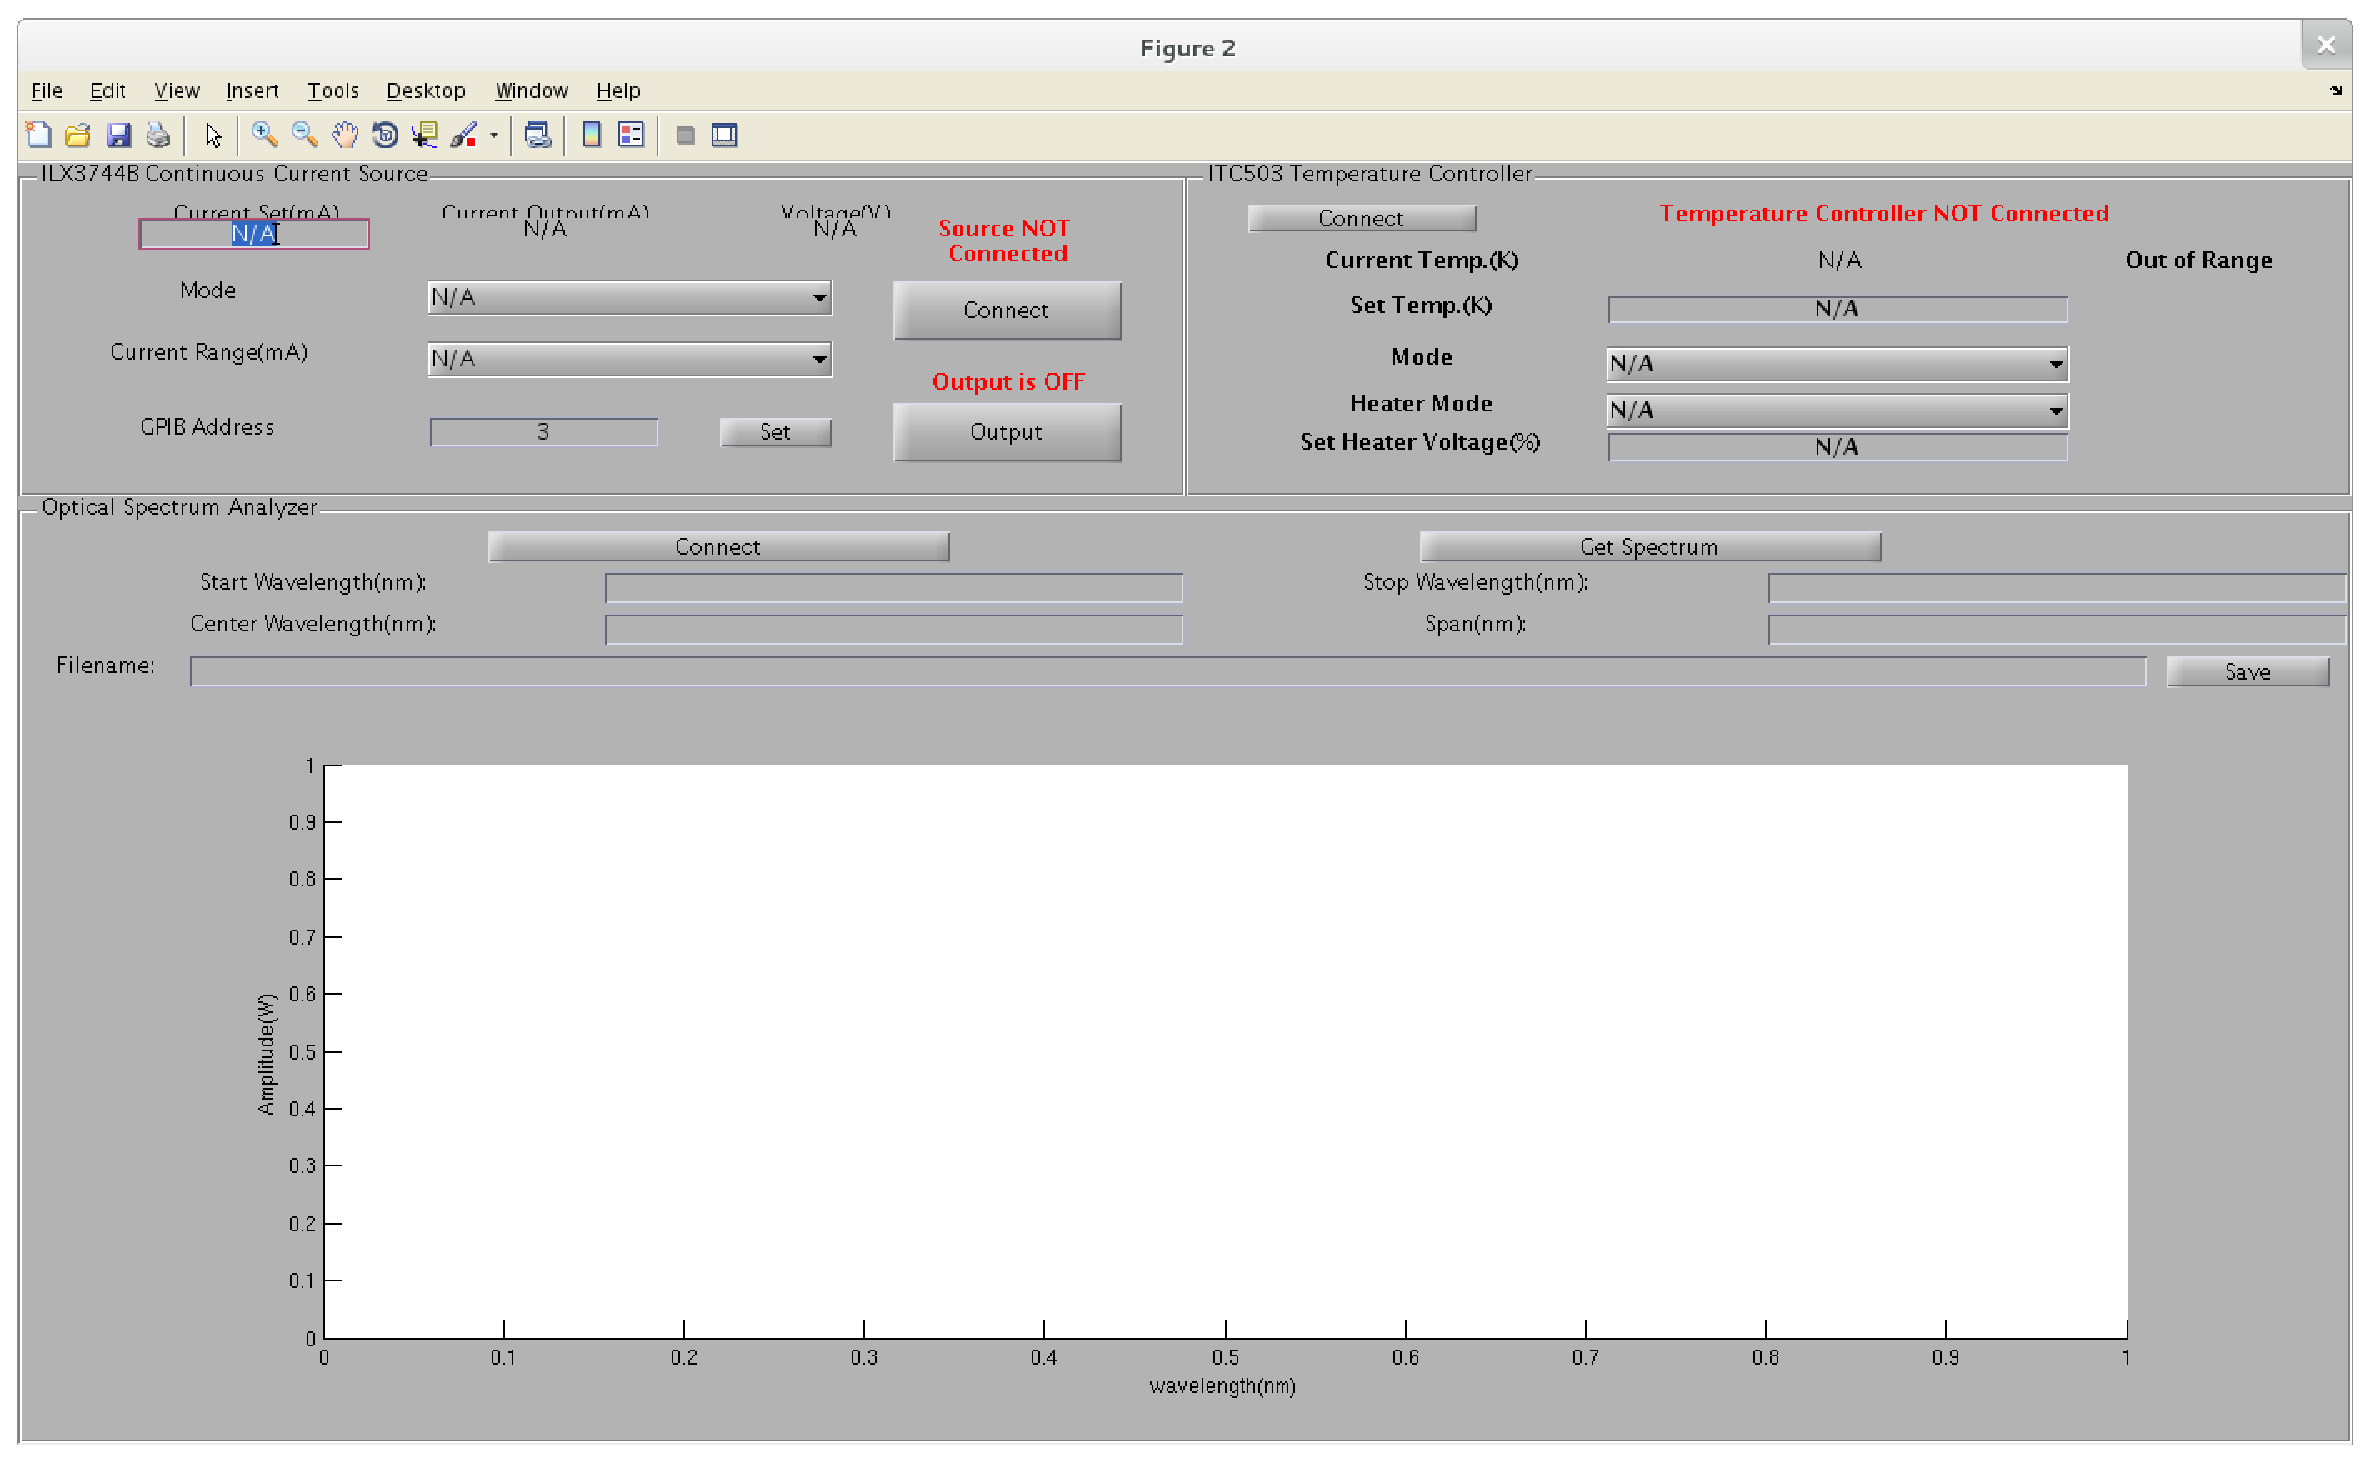
\includegraphics[width=0.9\textwidth]{./figs/main_window.eps}
	\caption{Main window}
	\label{fig:main_window}
\end{figure}

In the ``ILX3744B Continuous Current Source'' panel, the first text edit called
``Current Set'' is to set the output current. You should press ``enter'' button in
keyboard after the value is entered in this text edit to send the value to the
current source. The following two texts(``Current Output(mA)'', ``Voltage(V)'') show
the current and voltage information. These values will be updated periodically
when the communication is established. The red text ``Source NOT Connected'' shows
the connection status and it will change to green text ``Source Connected'' after
the connection is established. The button below is used to connect to the
current source. After clicked, if the connection is established, the text on the
button will change to ``Disconnect'' and used to disconnect the current source.
The red text ``Output is OFF'' shows the status of output enable. If the current
output is enabled by clicking the ``Output'' button below, the red text will
change to green text ``Output is ON''. There are two popup menus in this panel,
one is for the operation mode of current source and the other one is to set the
current range of current source. You can choose the proper one for your
measurement.

In the ``ITC503 Temperature Controller'' panel, the ``Connect'' button and red text
have the same function as mentioned above. The text bar below is used to show
the current temperature of the sensor which will be refreshed periodically when
connected. The text ``Out of Range'' shows the state of temperature stability.
Once the temperature is within 0.1K away from the set temperature, it will show
``Stable''. The text edit below is used to set temperature. You should press
``enter'' to confirm the set temperature. The ``Mode'' popup menu is used to show
the operation mode of the temperature controller. This parameter is to set how
you can operate the controller (remote or local) and whether to lock the front
panel of the controller (locked or unlocked). To have our gui remote controller
work, this has to be set as ``Remote\&Locked''. The popup menu below is used to
set the operation mode of heater and gas control. Since we don't have a gas
controller, the only thing that matters to us is the heater mode(Manual or
Auto). If the heater mode is set to be manual, the heater voltage below will be
used to set the heater power level. 

In the ``Optical Spectrum Analyzer'' panel, first there are two push buttons.
The ``Connect'' button is used to establish the connection to the OSA. The ``Get
Spectrum'' button is used to acquire the current spectrum from OSA and show this
spectrum in the axes below. There are four text edits named as ``Start
Wavelength'', ``Stop Wavelength'',``Center Wavelength'' and ``Span''. The
relation between these four values is as follows:
\begin{equation}
	\begin{aligned}
		\text{Center Wavelength} &= \frac{\text{Start Wavelength}+\text{Stop Wavelength}}{2}\\
		\text{Span} &=\text{Stop Wavelength}-\text{Start Wavelength}
	\end{aligned}
\end{equation}
When you change one of these values, the other three will be updated
automatically in both program and OSA. The ``Save'' button is used to save the
spectrum data in ``mat'' format with the filename defined by the ``filename''
text edit.

\end{document}

